\chapter{Results and Discussion}
\label{chapter:results} 
\noindent\rule{\linewidth}{2pt}

\section{Introduction}
This chapter discusses the experimental setup used for training and evaluating the proposed architecture on OCT image data. The experimentation involves training the autoencoder and CNN classification networks to improve their performance and get desired results. Training refers to the process with which the machine learns parameters which are involved in the computation of results.

\section{Experimental Setup}
A local computer system is used for the training of neural network. The device has a RAM of 8 GB and an SSD Disk Space of 512 GB. The processor is Intel Core i5 10th generation with an NVIDIA GeForce GTX 1650 GPU. The GPU is used for parallel computation which helps in accelerating the training speed and time of complex models. The programming is done with Python 3.9 and PyTorch version 1.13.

\subsection{Training setup for Autoencoder}
\vspace{1em}
The Autoencoder has the hyperparameter initialization as shown in Table \ref{table: auto}, which has been chosen for optimal performance.

\subsection{Training setup for Five-layered CNN}
\vspace{1em}
The Five-layered CNN has the  hyperparameter initialization as shown in Table \ref{table: CNN},  which has been chosen for optimal performance.
\newpage

\begin{table}[ht]
\centering
\caption{Parameter initialization for Autoencoder}
\renewcommand{\arraystretch}{2} 
\begin{tabular}{|c|c|}
\hline
\textbf{Parameter} & \textbf{Value/type} \\  \hline
Weight initialization & Random \\ \hline
Input size & 256 x 256 \\ \hline
Loss criterion & MSE Loss \\ \hline
Optimizer & Adam Optimizer \\ \hline
Learning rate & 1 x $10^{-3}$ \\ \hline
Batch size & 16 \\ \hline
\end{tabular}
\label{table: auto}
\end{table}

\begin{table}[ht]
\centering
\caption{Parameter initialization for Five-layered CNN}
\renewcommand{\arraystretch}{2} 
\begin{tabular}{|c|c|}
\hline
\textbf{Parameter} & \textbf{Value/type} \\ \hline
Weight initialization & Random \\ \hline
Input size & 128 x 128 \\ \hline
Loss criterion & MSE Loss \\ \hline
Optimizer & Adam Optimizer \\ \hline
Learning rate & 5.5 x $10^{-5}$ \\ \hline
Batch size & 16 \\ \hline
\end{tabular}
\label{table: CNN}
\end{table}

\subsection{Training setup for Bottleneck CNN}
\vspace{1em}
The Bottleneck CNN has the following hyperparameter initialization as shown in Table \ref{table: bottleneck} which has been chosen for optimal performance.
\newpage
\begin{table}[ht]
\centering
\caption{Parameter initialization for Bottleneck CNN}
\renewcommand{\arraystretch}{2} 
\begin{tabular}{|c|c|}
\hline
\textbf{Parameter} & \textbf{Value/type} \\ \hline
Weight initialization & Random \\ \hline
Input size & 128 x 128 \\ \hline
Loss criterion & MSE Loss \\ \hline
Optimizer & Adam Optimizer \\ \hline
Learning rate & 1 x $10^{-5}$ \\ \hline
Batch size & 16 \\ \hline
\end{tabular}
\label{table: bottleneck}
\end{table}

\section{Results}
The summary of the three proposed models for noise removal and classification are shown as follows:
\newpage

\begin{figure}[H]
\centering
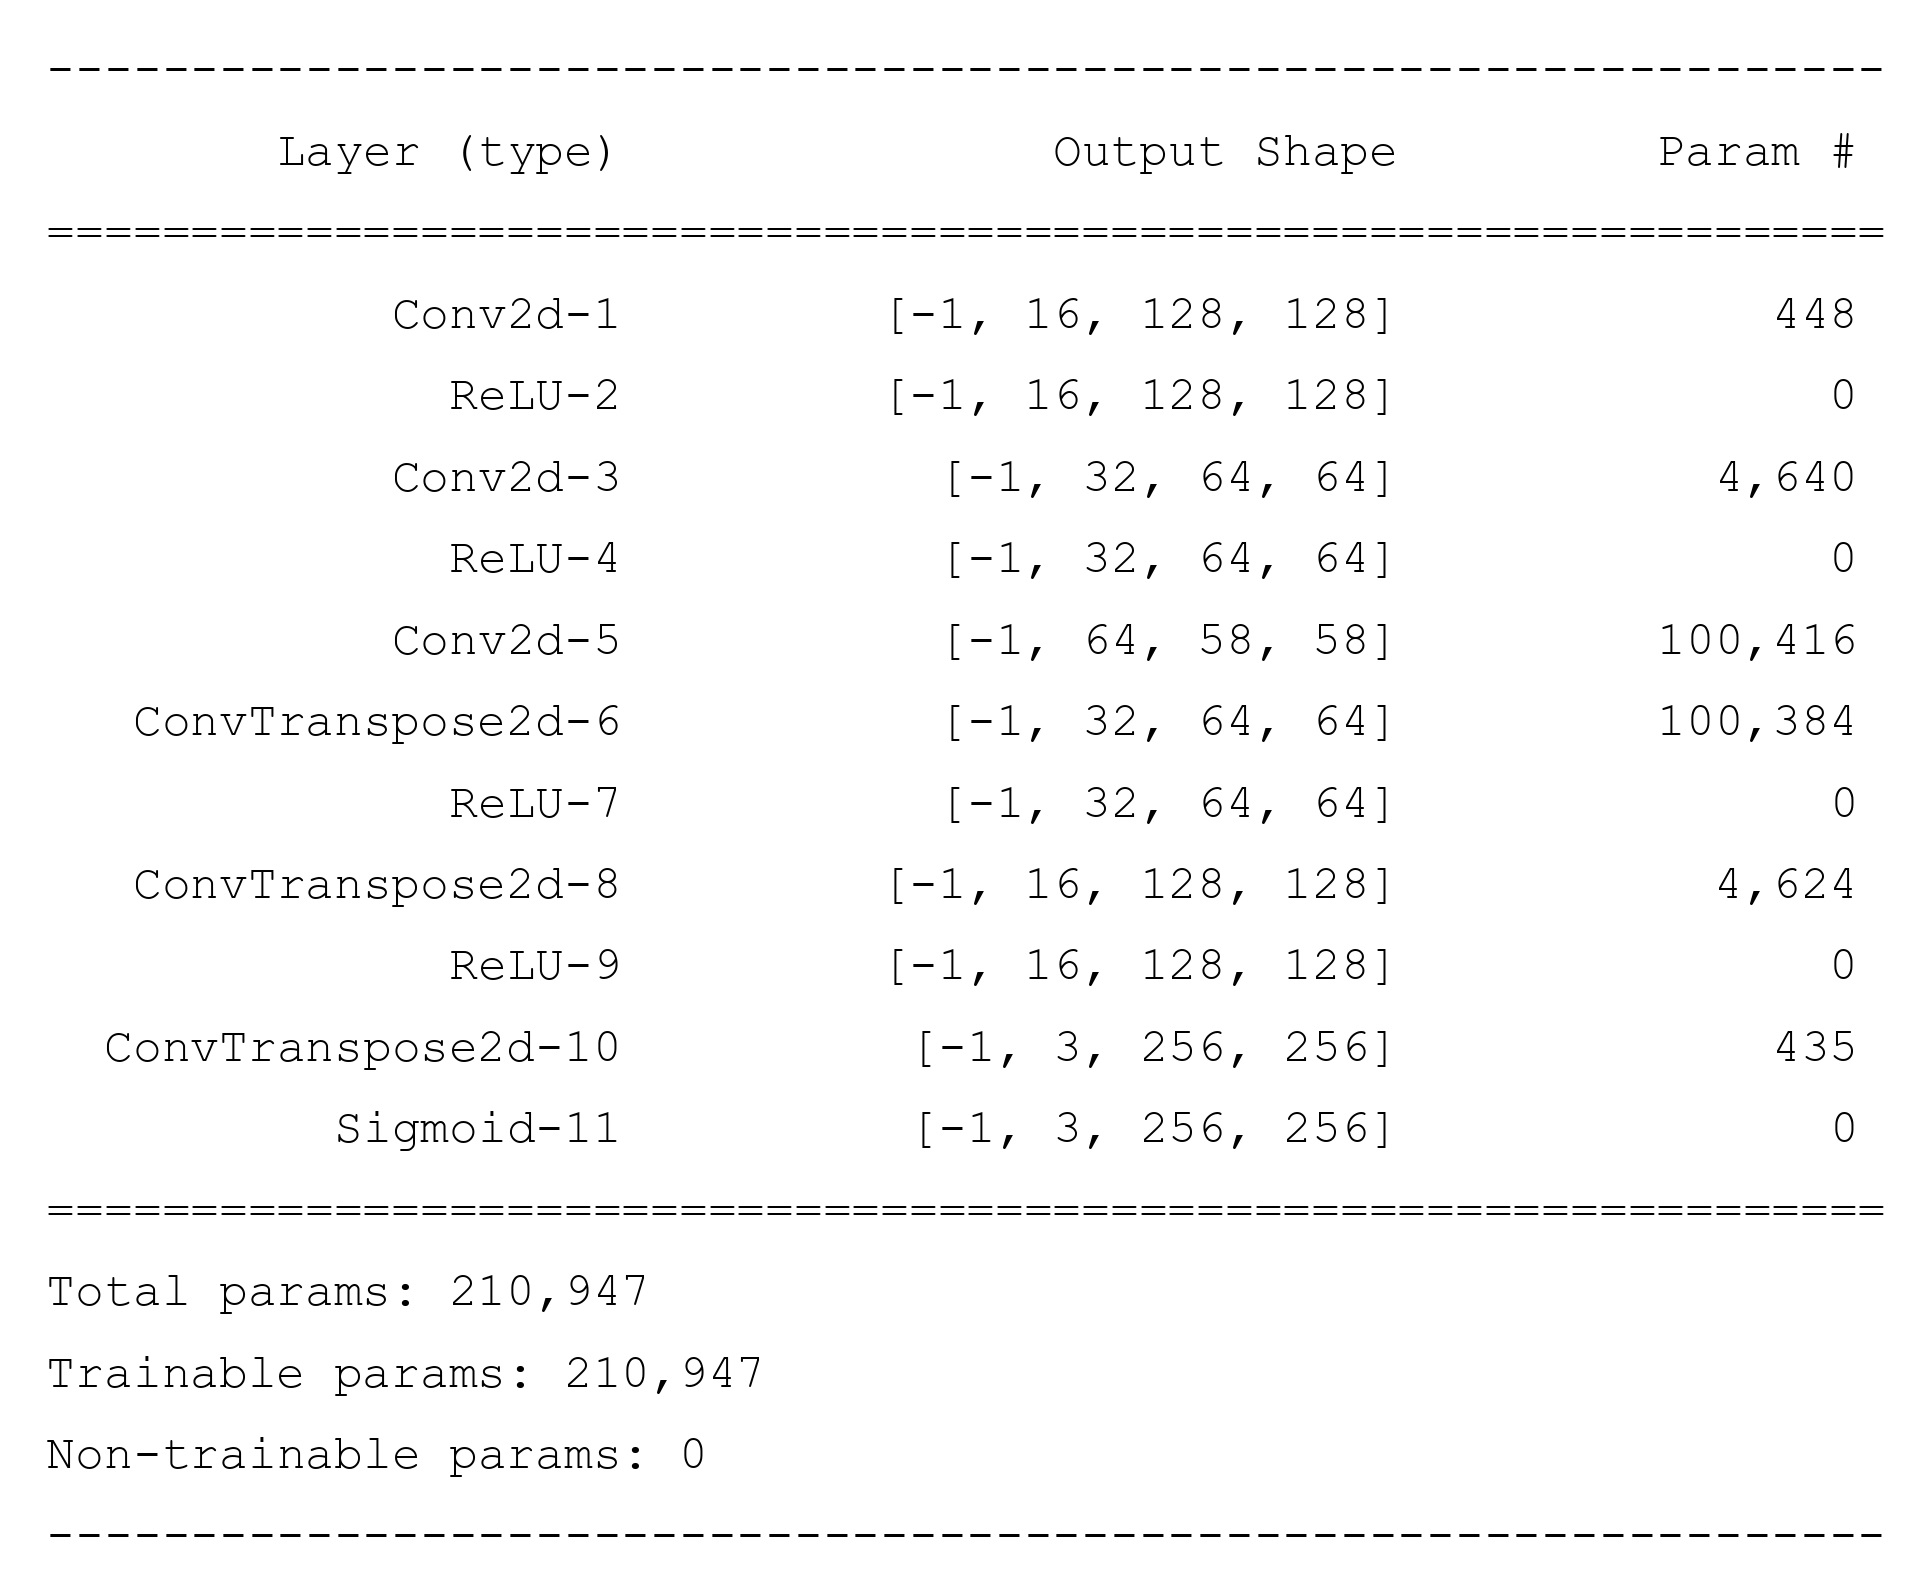
\includegraphics[width=\linewidth]{figimages/summaryAutoencoder.jpg}
\caption{Summary of Autoencoder model}
\label{fig: autoencoder summary}
\end{figure}


\begin{figure}[H]
\centering
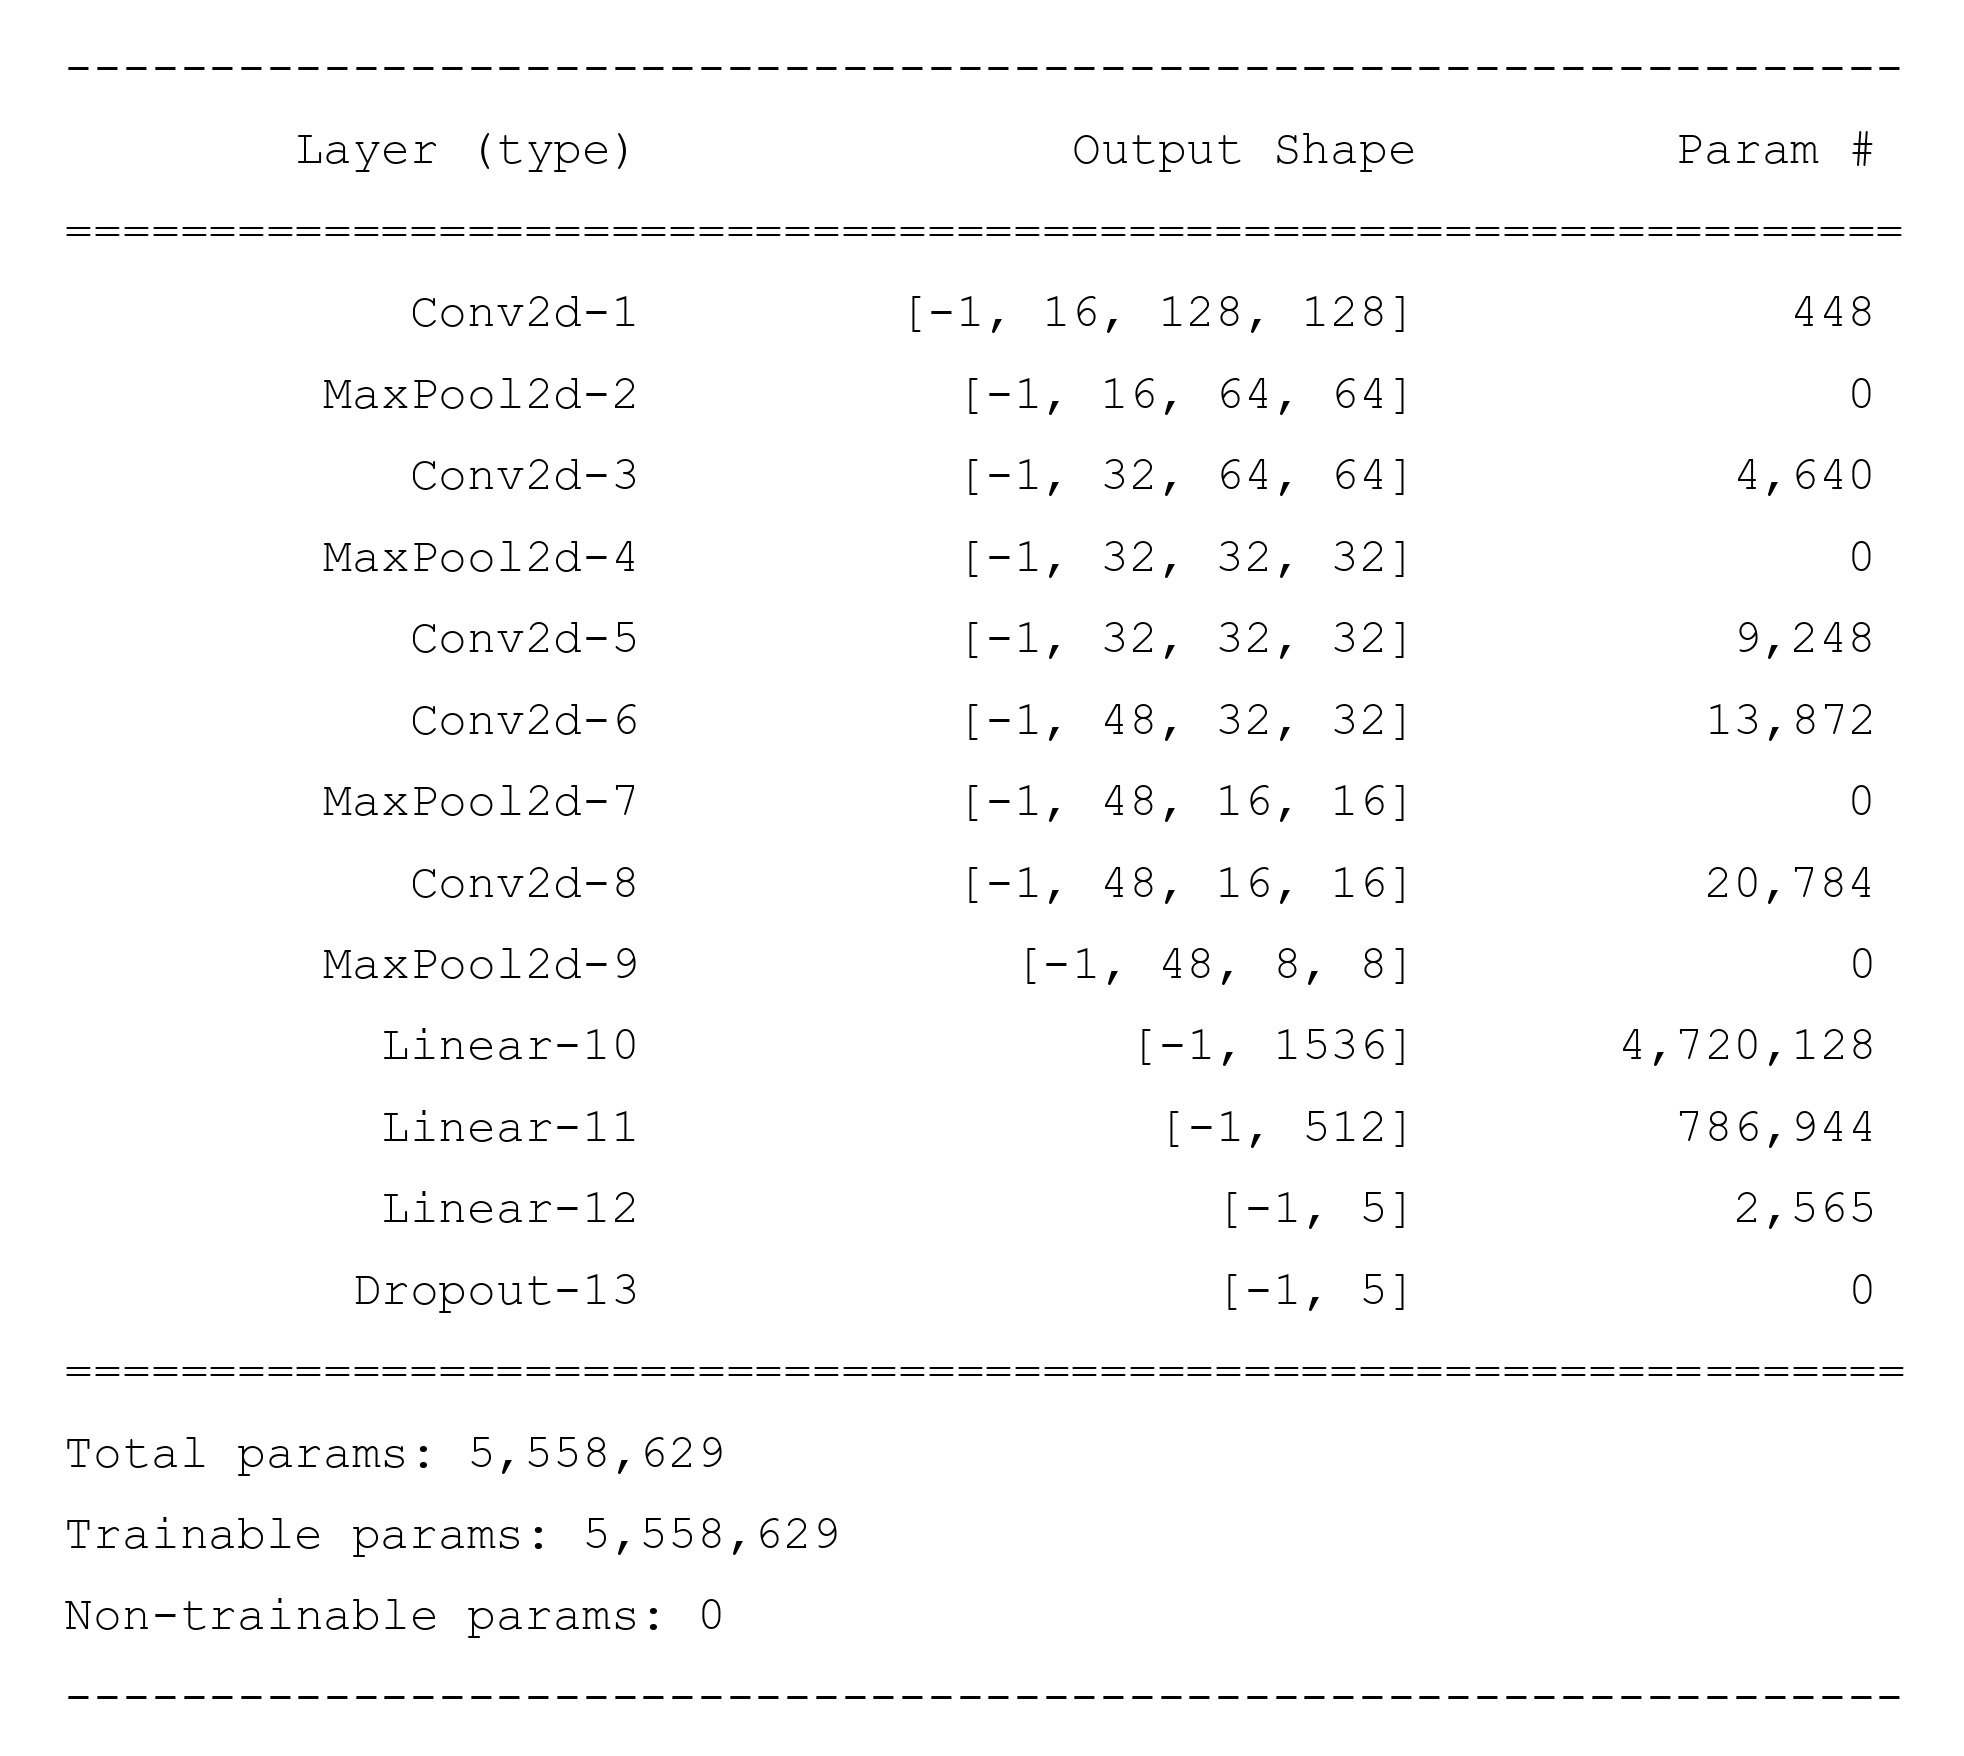
\includegraphics[width=\linewidth]{figimages/summary5Layered.jpg}
\caption{Summary of Five-layered CNN model}
\label{fig: 5CNN summary}
\end{figure}

\begin{figure}[H]
\centering
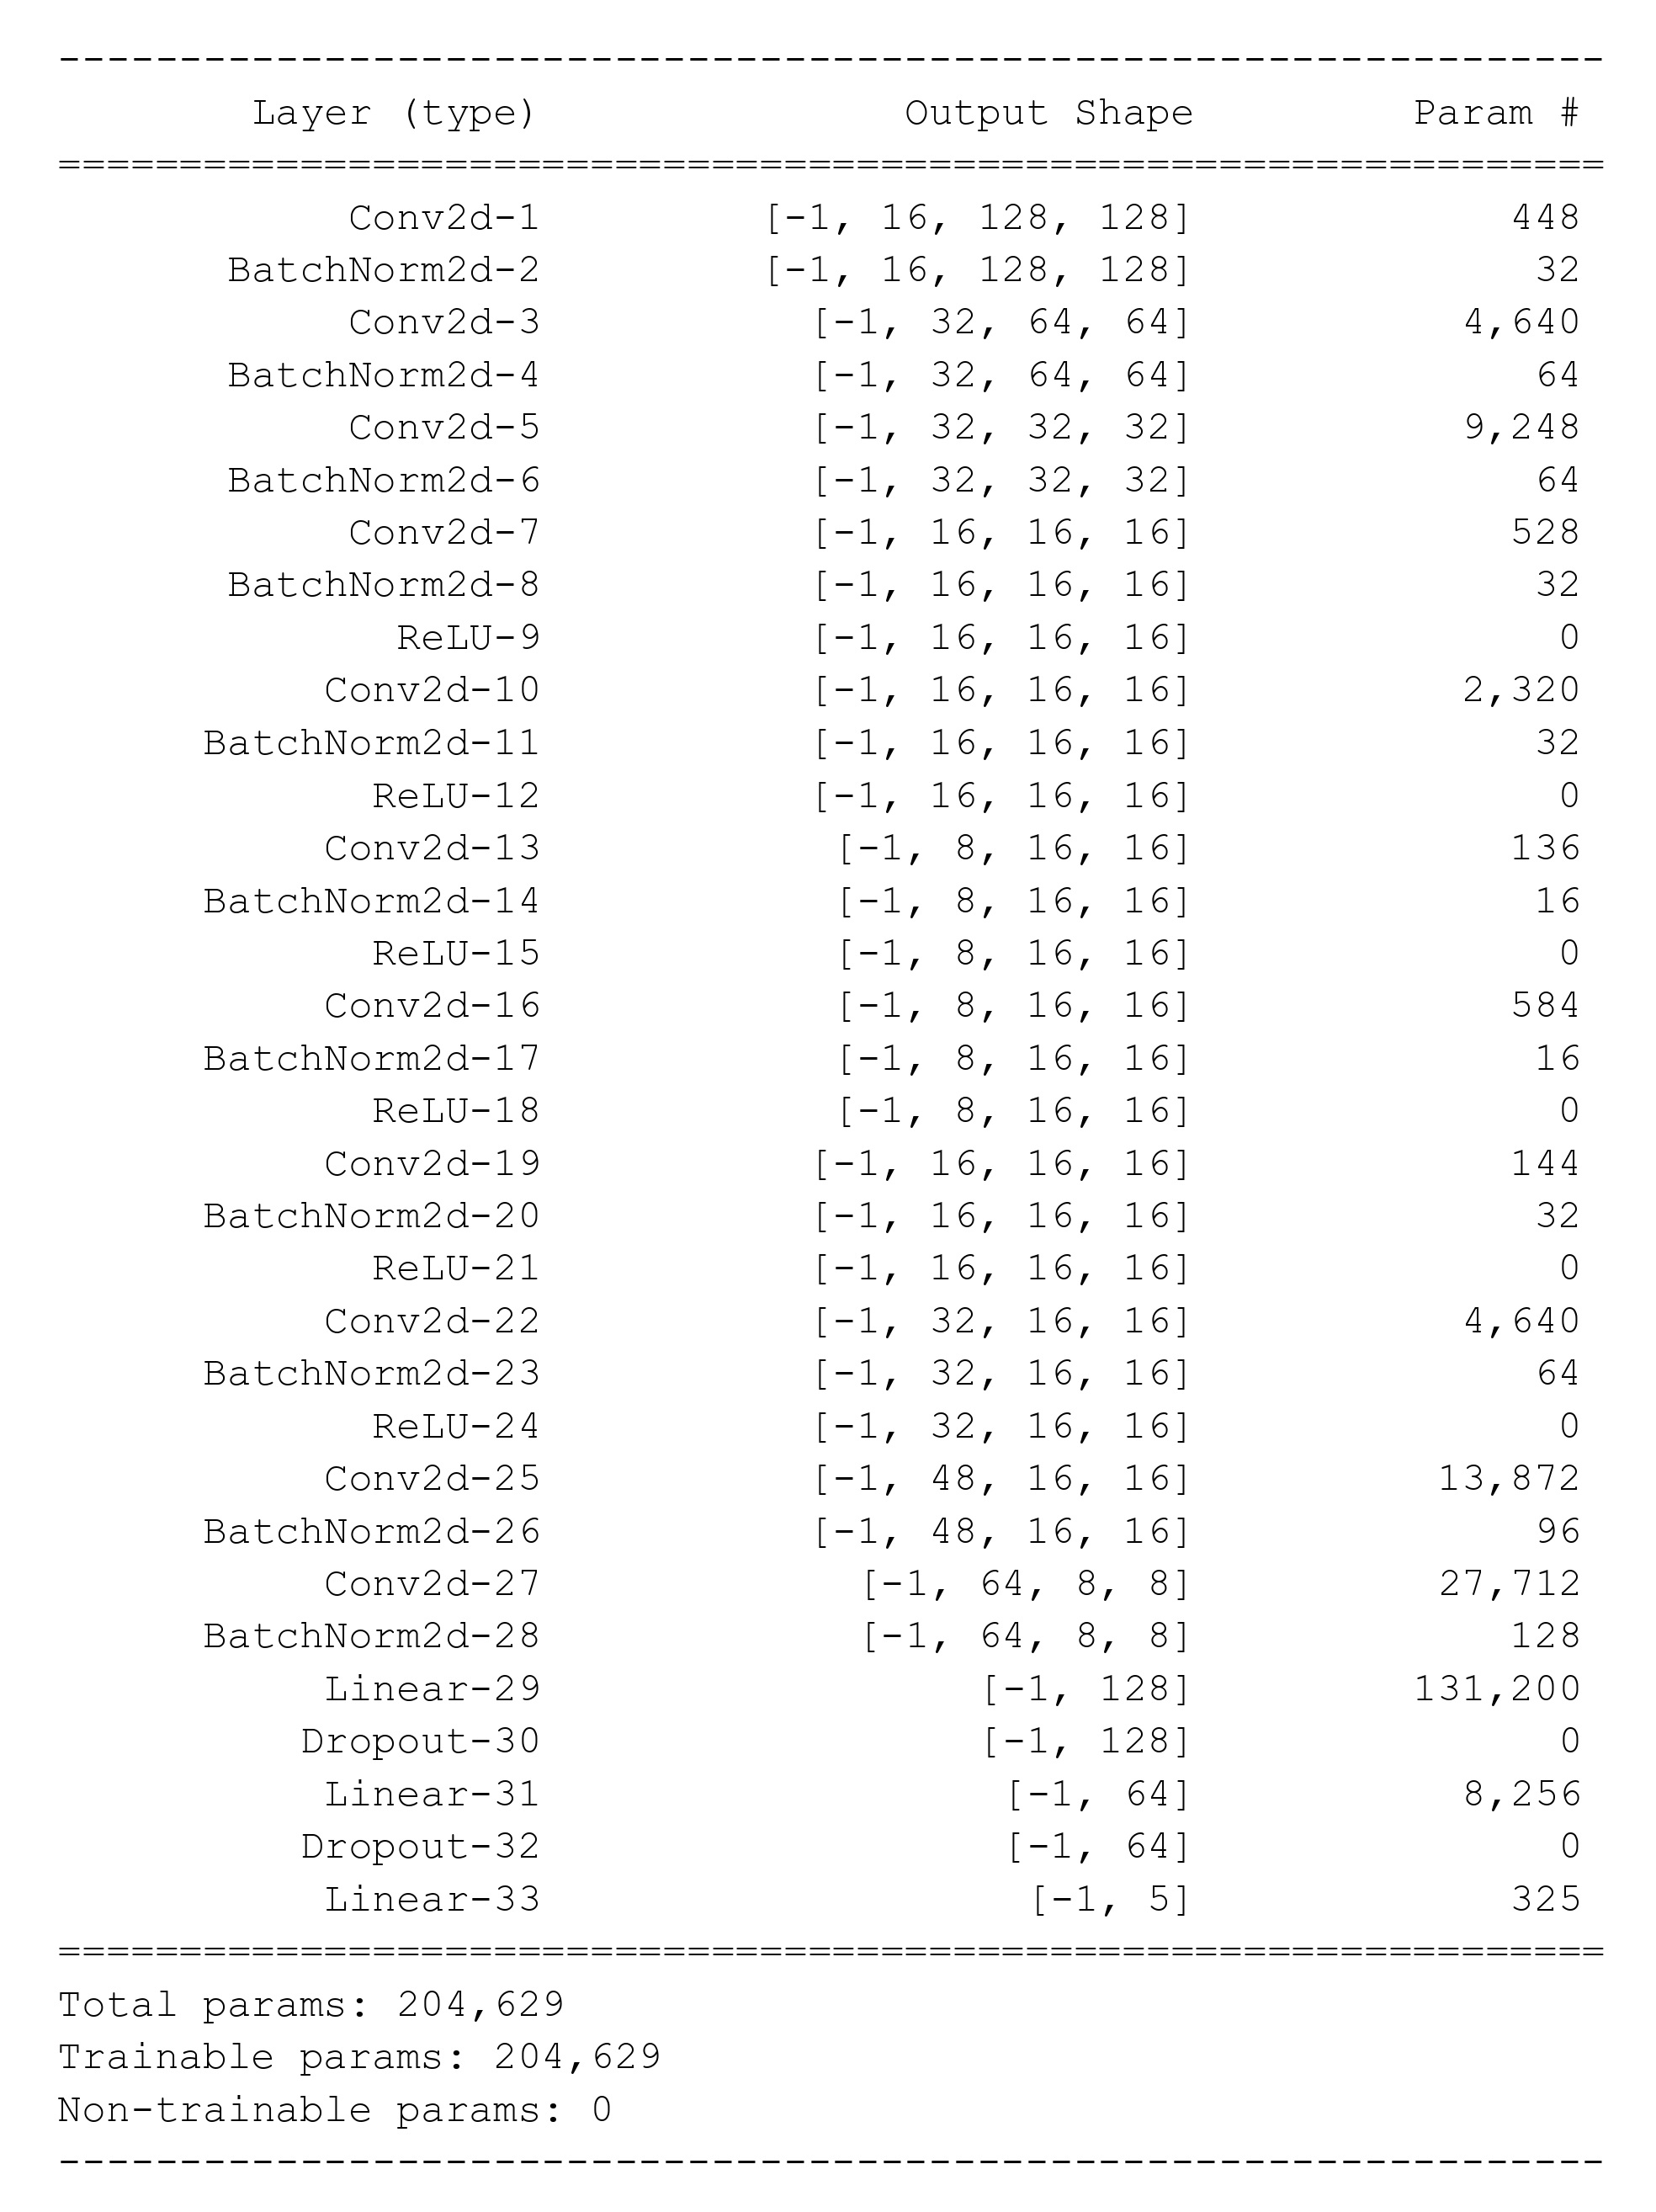
\includegraphics[width=\linewidth]{figimages/summaryBottleneck.jpg}
\caption{Summary of Bottleneck CNN model}
\label{fig: bottleneckSummary}
\end{figure}
\newpage

\subsection{Autoencoder}
\vspace{1em}
The PSNR and Mean Square Error plots during training of the Autoencoder have been shown in Figure \ref{fig: PSNR} and \ref{fig: MSE} respectively. The peak value of PSNR achieved is 27.324.

\begin{figure}[htb]
\centering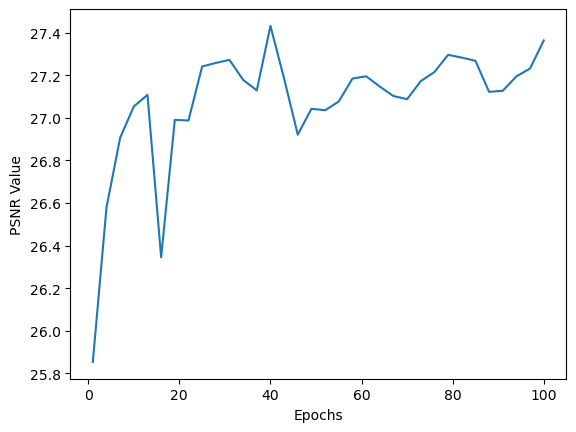
\includegraphics[width=0.7\linewidth]{figimages/PSNRplot.png}
\caption{PSNR Training Plot} 
\label{fig: PSNR}
\end{figure}

\begin{figure}[htb]
\centering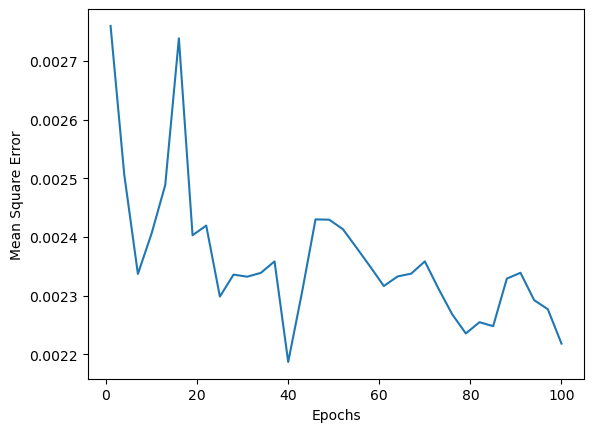
\includegraphics[width=0.7\linewidth]{figimages/MSEplot.png}
\caption{Mean Square Error plot during training} 
\label{fig: MSE}
\end{figure}

\par
The Figure \ref{fig: comparison} shows a comparison between the results obtained after noise removal and after applying the contrast adjustment using CLAHE on the denoised images.

\begin{figure}[htb]
\centering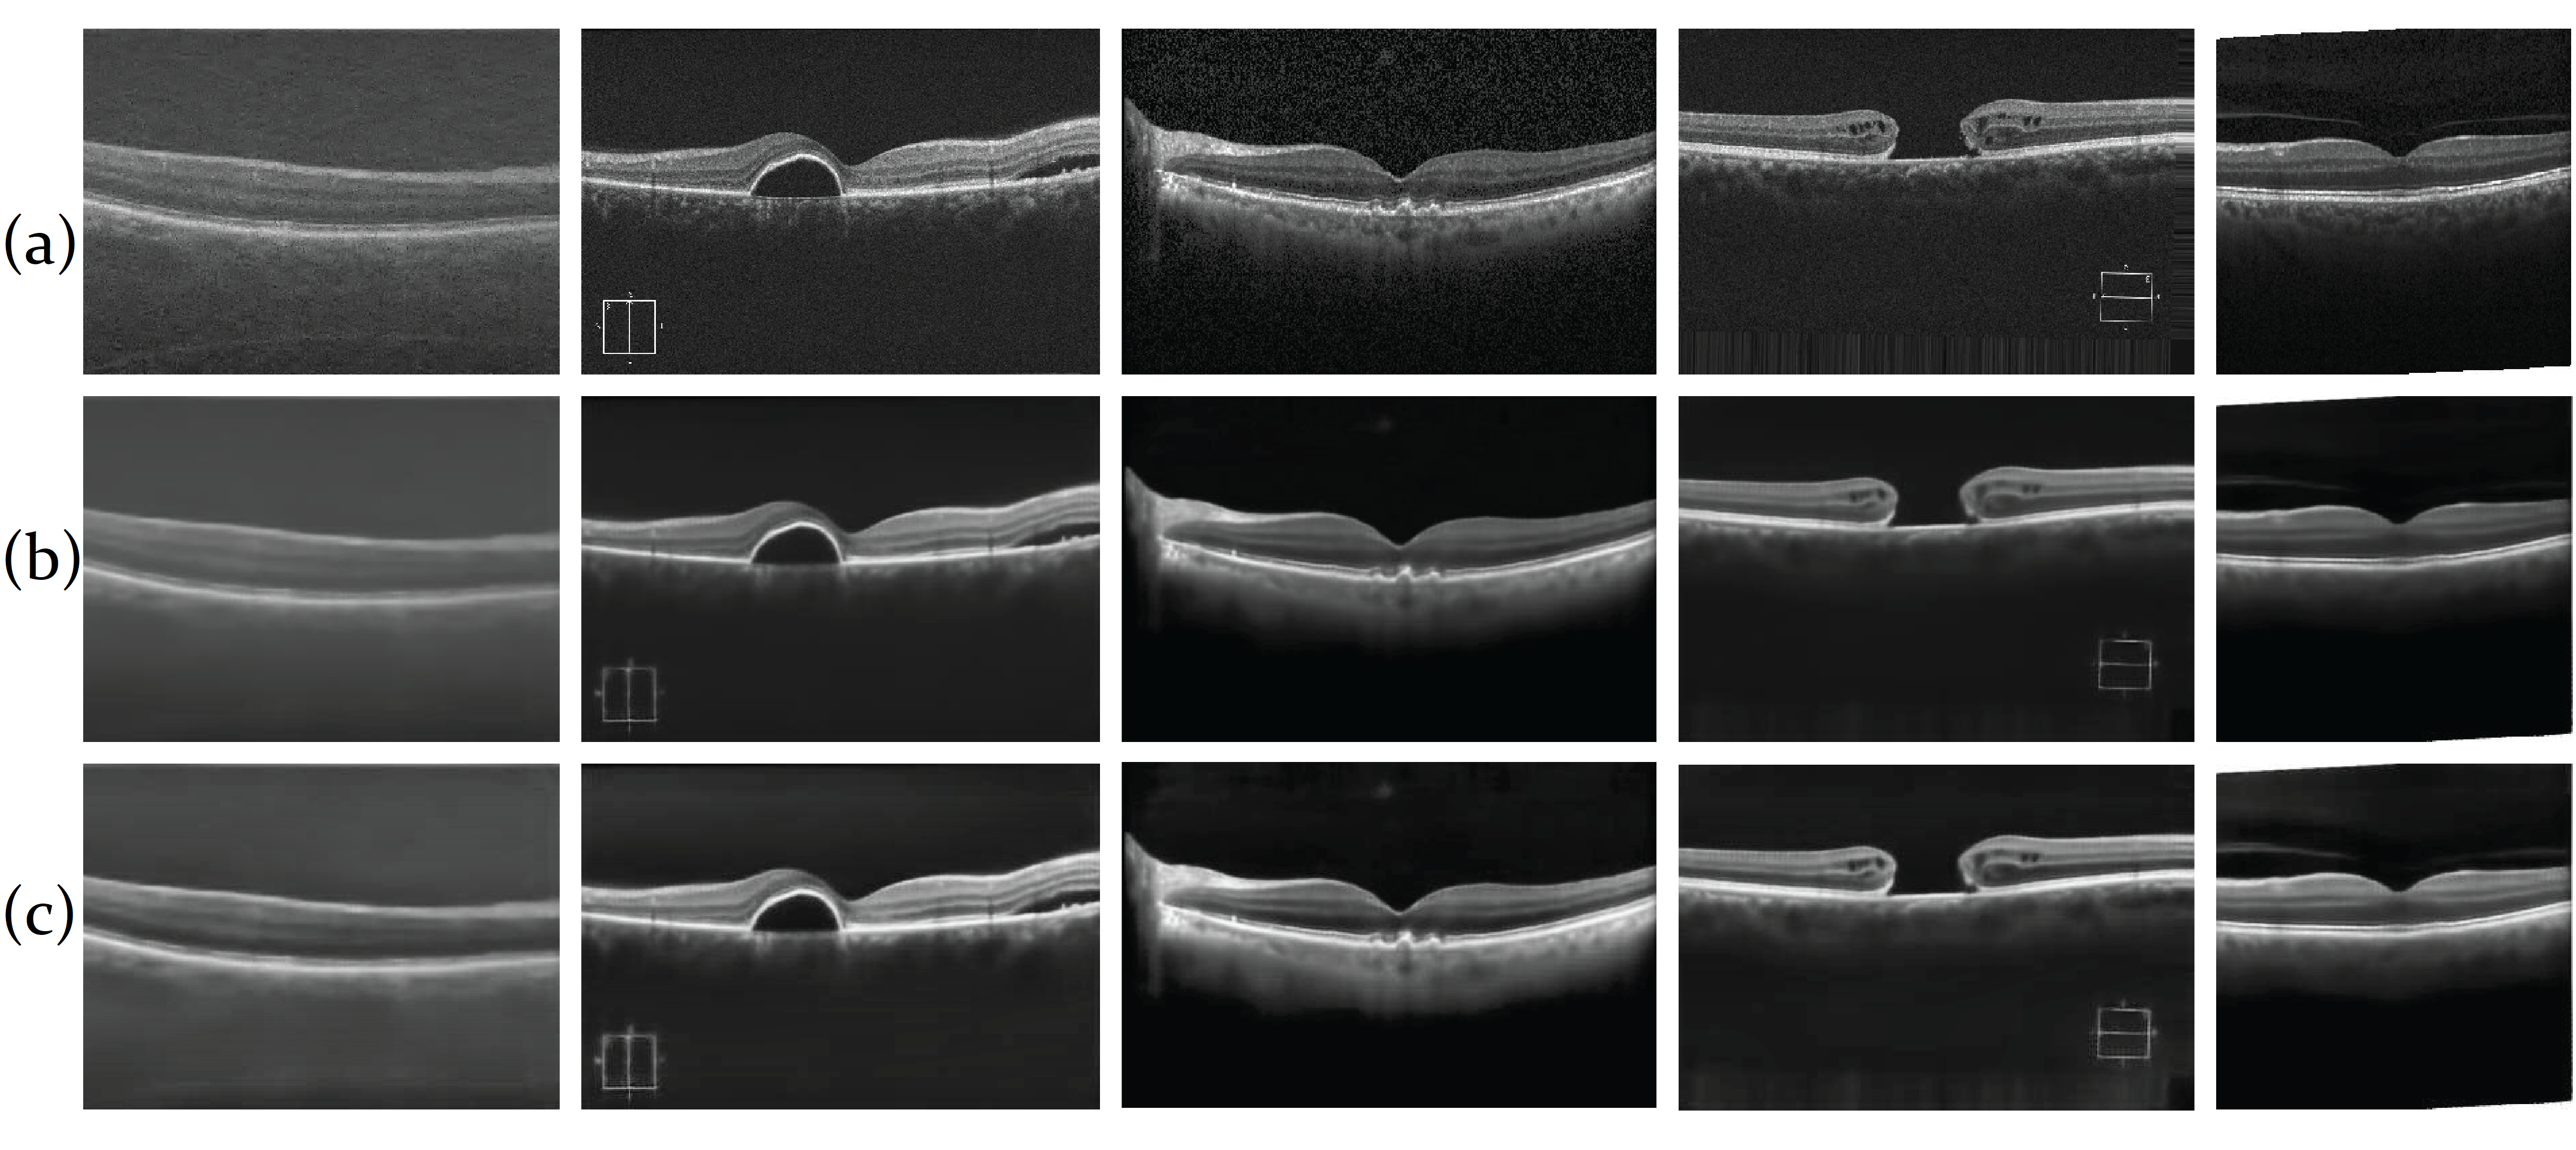
\includegraphics[width=\linewidth]{figimages/Comparison.png}
\caption{Comparison between (a) Raw images, (b) De-noised images and (c) Contrast Adjusted images} 
\label{fig: comparison}
\end{figure}

\subsection{Five-layered CNN}
\vspace{1em}
After successful training, various evaluation parameters have been set to judge the performance and validate the models. The Figure \ref{fig:trainingAcc5CNN} and \ref{fig:trainingLoss5CNN} show the plots from the training phase. 

\begin{figure}[htb]
\centering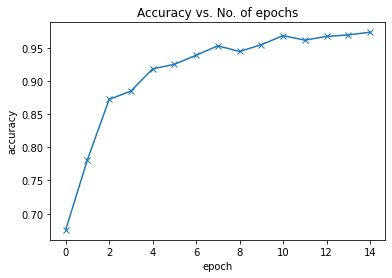
\includegraphics[width=0.75\linewidth]{figimages/acc5Layered.png}
\caption{Training Accuracy plot for Five-layered CNN} 
\label{fig:trainingAcc5CNN}
\end{figure}
\begin{figure}[htb]
\centering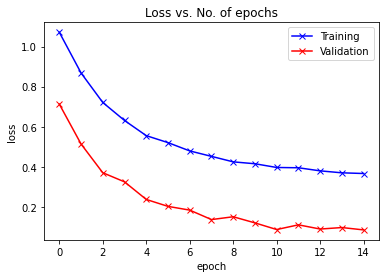
\includegraphics[width=0.75\linewidth]{figimages/loss5Layered.png}
\caption{Loss plot for Five-layered CNN} 
\label{fig:trainingLoss5CNN}
\end{figure}
\newpage

\par
The Five-layered CNN model achieves the highest validation accuracy of 97.33\% and minimum validation loss of 0.08. The F1 score calculated is 97.32. Table \ref{table: performance} shows the evaluation parameters including precision, recall, etc. The confusion matrix obtained for the same is shown in Figure \ref{fig:conf5CNN}.

\begin{table}[ht]
\centering
\caption{Performance parameters of the proposed classification models}
\renewcommand{\arraystretch}{2} 
\begin{tabular}{|c|c|c|}
\hline
\textbf{Parameter} & \textbf{Five-layered CNN} & \textbf{Bottleneck CNN} \\ \hline
Epochs & 15 & 15 \\ \hline
Learning Rate & 1 x $10^{-5}$ & 5.5 x $10^{-5}$ \\ \hline
Minimum Training Loss & 0.37 & 0.04 \\ \hline
Minimum Validation Loss & 0.08 & 0.07 \\ \hline
Maximum Validation Accuracy & 97.33\% & 97.50\% \\ \hline
Recall Accuracy (AMD) & 100\% & 100\% \\ \hline
Recall Accuracy (Normal) & 95.71\% & 99.71\% \\ \hline
Recall Accuracy (Drusen) & 94.28\% & 89.14\% \\ \hline
Recall Accuracy (CSR) & 97.14\% & 98.85\% \\ \hline
Recall Accuracy (MH) & 99.42\% & 99.71\% \\ \hline
Precision (AMD) & 99.43\% & 99.71\% \\ \hline
Precision (Normal) & 97.66\% & 96.67\% \\ \hline
Precision (Drusen) & 94.55\% & 98.42\% \\ \hline
Precision (CSR) & 94.97\% & 93.01\% \\ \hline
Precision (MH) & 100\% & 100\% \\ \hline
F1 Score & 97.32 & 97.46 \\ \hline
\end{tabular}
\label{table: performance}
\end{table}

\begin{figure}[H]
\centering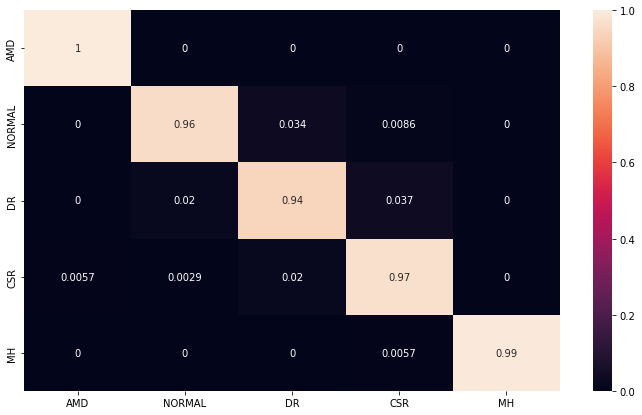
\includegraphics[width=0.75\linewidth]{figimages/confusion5Layered.png}
\caption{Confusion Matrix for Five-layered CNN} 
\label{fig:conf5CNN}
\end{figure}


\subsection{Bottleneck CNN}
\vspace{1em}
The Figure \ref{fig:trainingAccbottle} and \ref{fig:trainingLossbottle} show the plots from the training phase.

\begin{figure}[H]
\centering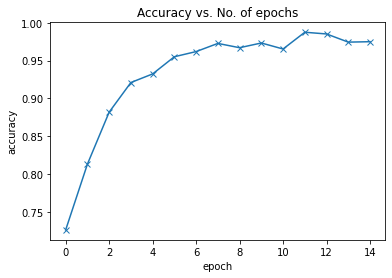
\includegraphics[width=0.75\linewidth]{figimages/accBottleneck.png}
\caption{Training Accuracy plot for Bottleneck CNN} 
\label{fig:trainingAccbottle}
\end{figure}

\begin{figure}[H]
\centering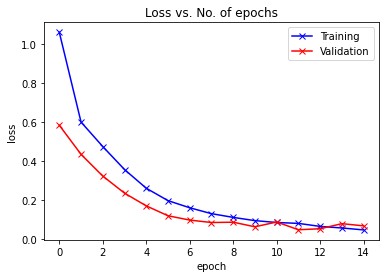
\includegraphics[width=0.75\linewidth]{figimages/lossBottleneck.png}
\caption{Loss plot for Bottleneck CNN} 
\label{fig:trainingLossbottle}
\end{figure}

The Bottleneck CNN model achieves the highest validation accuracy of 97.50\% and minimum validation loss of 0.07. The F1 score for the model is 97.46. Table \ref{table: performance} shows the evaluation parameters including precision, recall, etc. The confusion matrix obtained for the same is shown in Figure \ref{fig:confBottle}.

\begin{figure}[H]
\centering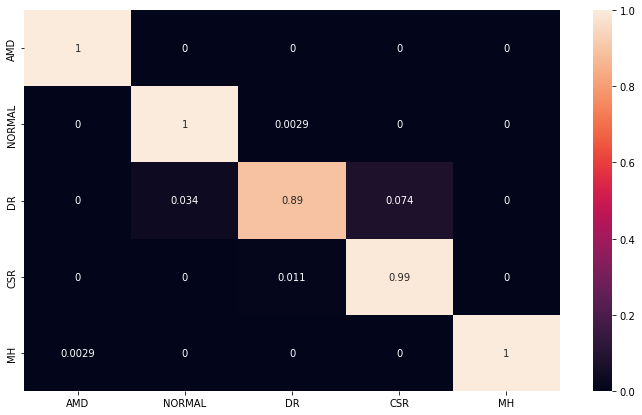
\includegraphics[width=0.75\linewidth]{figimages/confusionBottleneck.png}
\caption{Confusion Matrix for Bottleneck CNN} 
\label{fig:confBottle}
\end{figure}

\section{Discussion}
There have been different methods and algorithms used for classification of retinal diseases using OCT scans- raw, segmented, unsegmented etc. over the years. Some of the prominent research works are taken into consideration in this section.

\par
Hussain et al. \cite{Hussain2018} proposed a classification technique for OCT images of AMD and DME. The method involved image segmentation on the raw OCT scans before classification. The data was made of total 1,183 images consisting of 238 normal, 885 AMD, and 60 DME images. The method used Random Forest \cite{Breiman2001} algorithm for classification with a 95\% accuracy.

\par
Maetschke et al. \cite{Maetschke2019} devised a different approach with unsegmented raw OCT images. The technique consisted of a binary CNN classifier, classifying images of Glaucoma disease and normal eye. The data consists of 1,110 images with 263 healthy normal eye and 847 glaucoma effected images. The proposed method consists of five 3-D Convolutional layers with ReLU activation and Batch Normalization layers. The binary classifier had a 94\% accuracy.

\par
Feng et al. \cite{Li2019} devised a classification technique for DME, CNV, Drusen and normal eye classes. The data consists of a total 21,357 images. The data was classified using multi-ResNet50 ensemble. The proposed transfer learning method achieved an accuracy of 97.3\%.

\par
Tayal et. al.\cite{Tayal2022} proposed three novel CNN classifiers consisting of 5, 7 and 9 Convolutional layers respectively. The data consists of a total of 83,484 images. The best validation accuracy is achieved by 5-layered CNN model with an accuracy of 96.30\%. The images were denoised using median filters, contrast adjusted using CLAHE algorithm and fed to CNN classifier. The 4-class CNN is made of convolutional layers connected through pooling layers, followed by 3 linear layers and a 40\% dropout layer.

\par
Table \ref{table:discussion} demonstrates the efficacy comparison of existing techniques to the proposed approach. The proposed Bottleneck CNN along with denoising using Autoencoder outperforms the previous approaches by achieving an accuracy of 97.50\%.

\begin{table}[ht]
\centering
\caption{Comparison of performances of different methods with the proposed method}
\renewcommand{\arraystretch}{2} 
\begin{tabular}{|c|c|c|}
\hline
\textbf{Paper} & \textbf{Minimum Loss} & \textbf{Maximum Accuracy (\%)} \\ \hline
\cite{Li2019} & - & 97.30 \\ \hline
\cite{Tayal2022} & 0.15 & 96.30 \\ \hline
\cite{Maetschke2019} & - & 94 \\ \hline
\cite{Hussain2018} & - & 95 \\ \hline
Proposed & 0.07 & 97.50 \\ \hline
\end{tabular}
\label{table:discussion}
\end{table}

